\subsection*{Introduction}

For this exercise, we analyze a time series containing the British coal mining disasters under the time period 1851--1962. The difference between this exercise and the one in the course literature, is that we have a continuous time series as well as more than 1 \textbf{breakpoint}. A breakpoint is thus the year at which the intensity of the disasters change. We will use $d-1$ breakpoints, where $d$ then corresponds to the number of intervals we will use. In order to get a feel for the time series we will analyze, a figure containing a histogram of the disasters is found in figure \ref{fig:disasters}.

\begin{figure}[H]
  \centering
    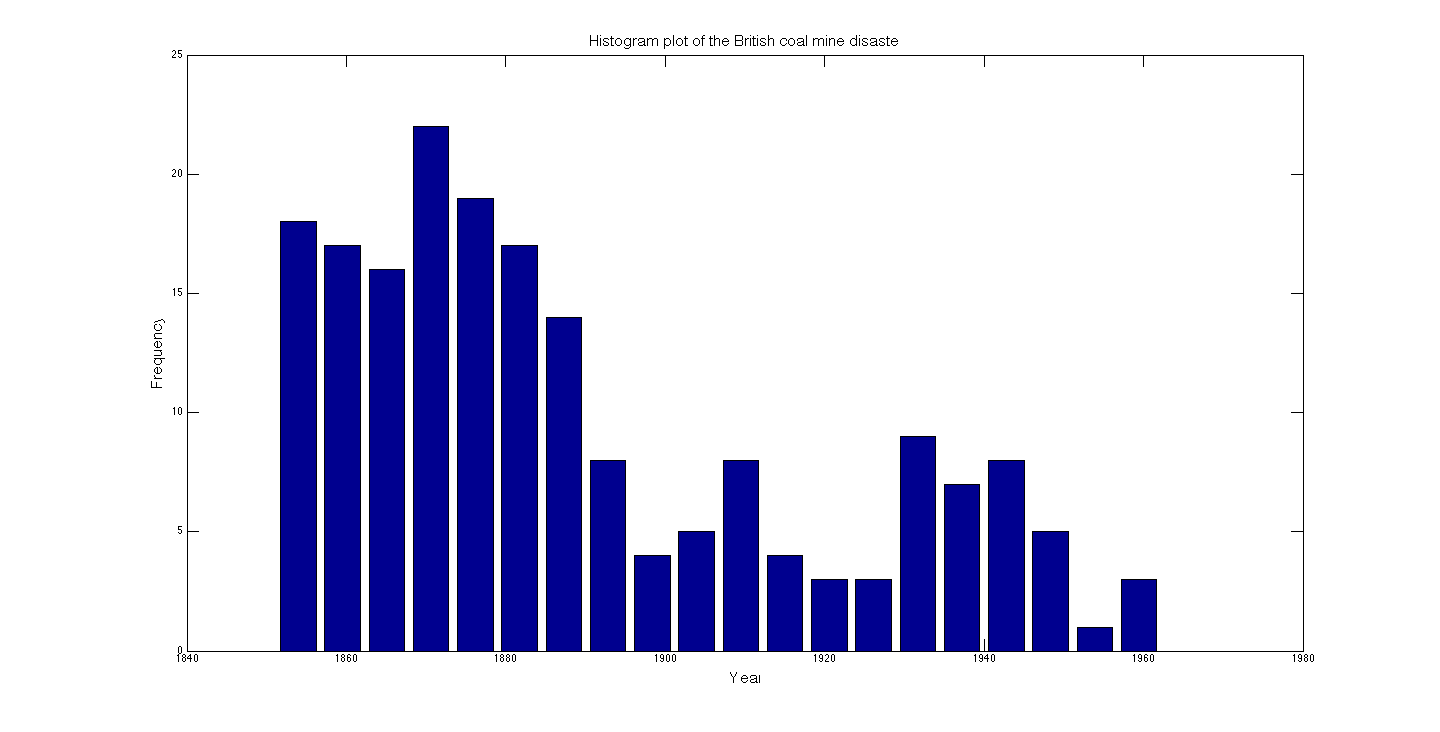
\includegraphics[scale=0.24]{./Figures/disasters.png}
  \caption[An Electron]{Histogram plot of the British coal mine disasters in the time period 1851--1962.}
  \label{fig:disasters}
\end{figure}

As is seen in figure \ref{fig:disasters} there is a change in the disaster intensity at the turn of the century, perhaps due to some legislation regarding work safety or some technological advancement. \\ \\ To begin the exercise, we define the vector $\boldsymbol{t}$ to be the vector containing all of the breakpoints $t_i, \: i = 2,\dots d$ aswell as the start and end point $t_1 = 1851$ and $t_{d+1}=1963$. We wish to model the disasters using an inhomogenous Poisson process with an intensity $\lambda_i$ for each of the intervals $[t_i,t_{i+1}), \: i = 1,\dots,d$. Where all of the $\lambda_i$'s are collected in a vector $\boldsymbol{\lambda}$. \\ We will denote the time series containing the year at which disaster struck as $\boldsymbol{\tau} = (\tau_1,\dots,\tau_n)$ for $n = 191$, where the subscript denotes accident $i$. \\ We then define the number of accidents under the interval $[t_i,t_{i+1})$ to be
\[n_i(\boldsymbol{\tau}) = \sum^n_{j = 1}\mathbbm{1}\{[t_i,t_{i+1})\}\cdot \tau_j \]
We set a $\Gamma(2,\theta)$ prior on the intensities, $\lambda_i$, and a $\Gamma(2,\beta)$ hyperprior on $\theta$. Where $\beta$ is a hyperparameter that needs to be specified. Furthermore, we put the prior
\[ f(\boldsymbol{t}) \propto\left\{
	\begin{array}{l}
		\prod^d_{i = 1}(t_{i+1} - t_i), \quad \text{for } t_1 < t_2 < \dots < t_{d+1} \\
		0, \quad \text{else} 
	\end{array}
\right. \]
 This prior prevents the breakpoints from being located to closely. All of these prior assumptions then imply that 
\[f(\boldsymbol{\tau} | \boldsymbol{\lambda}, \boldsymbol{t}) \propto \prod^d_{i = 1}\lambda_i^{n_i(\boldsymbol{\tau})}\cdot\exp \left \{ - \sum^d_{i = 1}\lambda_i(t_{i+1} - t_i) \right \} \]
In order to sample from the posterior $f(\theta,\boldsymbol{t},\boldsymbol{\lambda} | \boldsymbol{\tau})$ we will construct a hybrid \textbf{M}arkov \textbf{C}hain \textbf{M}onte \textbf{C}arlo algorithm, where the hybrid comes from the fact that we will need to sample $\boldsymbol{t}$ using a Metropolis--Hastings step whereas the other components can be updated using a Gibbs sampler. \\ \\ There are several ways to choose the proposal distribution for the Metropolis--Hastings, we chose to use the \textit{Random walk proposal}, which means that we will update one breakpoint at a time and for each breakpoint $t_i$ generate a candidate $t^*_i$ according to
\[t^*_i = t_i + \epsilon, \quad \epsilon \sim \text{Unif}(-R,R) \]
Where $R = \rho(t_{i+1} - t_{i-1})$ and $\rho$ is a tuning parameter.

%Basic idea of MCMC (Markov Chain Monte Carlo): To sample from a density f we construct a
%Markov chain having f as stationary distribution. A law of
%large numbers for Markov chains guarantees convergence. \\

%MCMC is widely used for sampling, due to its simplicity when dealing with complex distributions or distributions of high dimensions. However, the price is that the samples will be statistically dependant. It can be used to simulate a probabiltiy distribution $\pi(x)$ that is known only up to a normalizing constant, which is especially important in Bayesian inference with $\pi$ as the posterior distribution.
